\documentclass[7pt]{beamer}


\usepackage[utf8]{inputenc}
\usepackage[T2A]{fontenc}
\usepackage[english,russian]{babel}
\usepackage{amsmath}
\usepackage{amssymb}
\usepackage{amsfonts}
\usepackage{verbatim}
\usepackage{graphicx}
\usepackage{wrapfig}
\usepackage{mathtools}
\usepackage{float}
\usepackage{animate}
\usepackage{movie15}
\usepackage[font=small]{caption}
%\usepackage[left=3cm,right=2cm,top=2cm,bottom=2cm,bindingoffset=0cm]{geometry}
%\usepackage[greekit,hyperref,remarks,footwhole]{fn2kursstyle}

\graphicspath{{legacy/}, {../pic/}}

\addto\captionsrussian{\renewcommand{\refname}{Список использованных источников}}
\setbeamertemplate{footline}[frame number]
\DeclareMathOperator{\re}{Re}
%\renewcommand{\baselinestretch}{1.5}
%\setlength{\parindent}{12.5mm}

\captionsetup[figure]{name=Рис.}
\frenchspacing
\righthyphenmin=2
\numberwithin{equation}{section}
\newcommand{\eps}{\ensuremath{\varepsilon}}
\newcommand{\ddfrac}[2]{\ensuremath{\frac{d^2 x_{#1}}{d {#2}^2}}}
\newcommand*{\Scale}[2][4]{\scalebox{#1}{$#2$}}
\newcommand*{\Resize}[2]{\resizebox{#1}{!}{$#2$}}
\renewcommand{\phi}{\ensuremath{\varphi}}

\usepackage{caption}
\DeclareCaptionFont{xxviii}{\fontsize{10}{9}\selectfont}
\captionsetup{font=xxviii}

\mode<presentation>{
\usetheme{Frankfurt} %тема с таблицей разделов и подразделов

\useinnertheme{circles}   %внутренняя тема
\useoutertheme{smoothbars}   %внешняя тема
\usecolortheme{crane}     %цветовая схема
\usefonttheme{serif}}    %шрифты

\def\Arsh{\mathop{\mathrm{Arsh}}}

\title{Метод конечных элементов в задаче моделирования прогиба балки}
\author{Студент: Касьянова К.\,А., ФН2-61Б\\ \vspace*{5mm}
Научный руководитель: к.ф-м.н., доцент кафедры ФН-2 Марчевский~И.\,К.}
\date{\today}
\titlegraphic{
\includegraphics[width=2cm]{emblema}}

\begin{document}
\mathtoolsset{showonlyrefs} 

\begin{frame}[plain]
	\maketitle
\end{frame}

\section{Точное решение дифференциального уравнения, описывающего форму упругой линии балки}

\begin{frame}{Точное решение дифференциального уравнения, описывающего форму упругой линии балки} 
	\begin{block}{Уравнение, описывающее прогиб балки:}
	\[(EIy^{''}_{zz})^{''}_{zz}=q,\]
	\end{block}	
	где $E$ --- модуль упругости балки; $I$ --- момент инерции относительно поперечной оси; $q$ --- распределённая внешняя нагрузка, действующая на балку. \\
 
	\begin{block}{Граничные условия:}
		\begin{enumerate}
		\item $y|_{z=z_{0}}=y_{0}$ --- заданная величина прогиба;
		\item $y'|_{z=z_{0}}=y'_{0}$ --- заданный угол поворота сечения;
		\item $EIy''|_{z=z_{0}}=M_{0}$ --- изгибающий момент;
		\item $EIy'''|_{z=z_{0}}= Q_{0}$ --- перерезывающая сила.
		\end{enumerate}
	\end{block}	
\end{frame}

\section{Метод конечных элементов}
\begin{frame}{Метод конечных элементов}
	\begin{block}{Рассмотрим слабую постановку задачи о прогибе (метод Галёркина):}
		\begin{equation}
			\label{beamm}
			\Scale[0.98]{\int\limits_{0}^{L}w\frac{d^{2}}{dz^{2}}(EI\frac{d^{2}u}{dz^{2}})dz=\int\limits_{0}^{L}wqdz,}
		\end{equation}
	где $w$ --- произвольная пробная функция, принадлежащая классу $W_{2}^{2}[0,L]$.
	\end{block}

	Полученное выражение два раза интегрируем по частям: 
	\begin{block}{}
	\[
		\Scale[0.98] {
			w\frac{d}{dz}(EI\frac{d^{2}u}{dz^{2}})\bigg|_0^L-\int\limits_{0}^{L}\frac{dw}{dz}\frac{d}{dz}(EI\frac{d^{2}u}{dz^{2}})dz=\int\limits_{0}^{L}wqdz,
		}
	\]
	\[
		\Scale[0.98] {
			w\frac{d}{dz}(EI\frac{d^{2}u}{dz^{2}})\bigg|_0^L-\frac{dw}{dz}(EI\frac{d^{2}u}{dz^{2}})\bigg|_0^L+\int\limits_{0}^{L}EI\frac{d^{2}w}{dz^{2}}\frac{d^{2}u}{dz^{2}}dz=\int\limits_{0}^{L}wqdz.
		}
	\]
	\end{block}
\end{frame}


\begin{frame}{}
	При решении задачи на прогиб двухузловой элемент имеет вид:
	\begin{figure}[h]
		\centering
		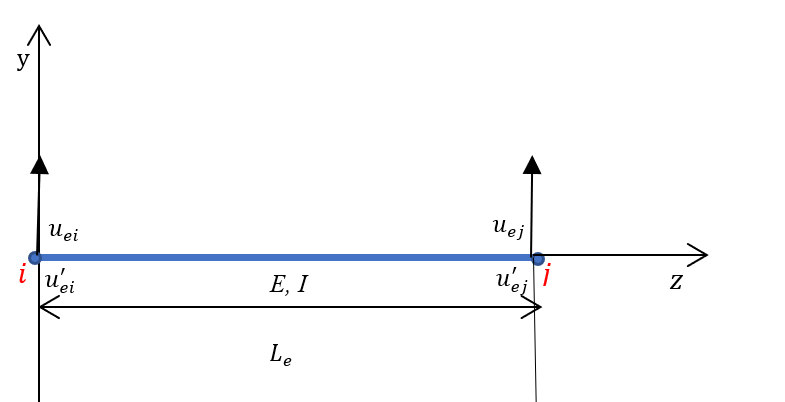
\includegraphics[width=0.55\textwidth]{element}
		\label{fig:element}
	\end{figure}
		
	\begin{block}{Рассмотрим выражение для функции формы и его производной для элемента:}
		\[u_e(z)=N_{1e}u|_i + N_{2e}\frac{du}{dz}\Bigr|_i+N_{3e}u|_{i+1} + N_{4e}\frac{du}{dz}\Bigr|_{i+1},\]
		\[\frac{du_e}{dz}=\frac{dN_{1e}}{dz}u|_i+\frac{dN_{2e}}{dz}\frac{du}{dz}\Bigr|_i+\frac{dN_{3e}}{dz}u|_{i+1}+\frac{dN_{4e}}{dz}\frac{du}{dz}\Bigr|_{i+1}.\]
	\end{block}
\end{frame}

\begin{frame}{}
	Из условий:
		\[u_e(0)=u|_i, u_e^{'}(0)=u^{'}|_{i}, u_{e}(L_e)=u|_{i+1}, u_{e}^{'}(L_e)=u^{'}|_{i+1},\] 
	получаем функции формы $N_{1e},N_{2e},N_{3e},N_{4e}$:
	\begin{block}{} 
		\begin{equation}
			\label{beam1}
			N_{1e}(z)=\frac{(L_e-z)^2(L_e+2z)}{L_e^3},~~ N_{2e}(z)=\frac{z(L_e-z)^{2}}{L_e^{2}},
		\end{equation}
		\begin{equation}
			\label{beam2}
			N_{3e}(z)=\frac{z^{2}(3L_e-2z)}{L_e^3},~~N_{4e}(z)=\frac{z^2(z-L_e)}{L_e^{2}}.
		\end{equation}
	\end{block}

	\begin{figure}[H]
		\centering
		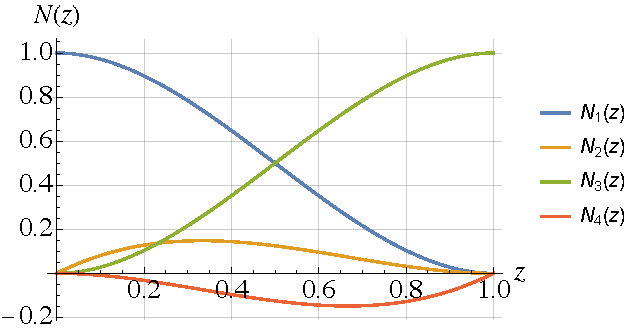
\includegraphics[width=0.5\textwidth]{2_formfunctions}
		\caption{Функции формы для двухузлового элемента}
		\label{fig:hermite}
	\end{figure}
\end{frame}
	
\begin{frame}
Выражение (\refeq{beam1}) для функции $u_{e}$ можем записать для одного элемента в следующем виде:
	\begin{block}{}
		\[
			u_e(z)=\textbf{N}_e \textbf{u}_{e}=
			\left[
			\begin{array}{cccc}
				N_{1e}(z) & N_{2e}(z) & N_{3e}(z) & N_{4e}(z)
			\end{array}
			\right]
			\Scale[0.7] {
				\left\{
				\begin{array}{ccc}
					u_{1}   \\
					u^{'}_{1}  \\
						u_{2}\\
						u^{'}_{2}\\
				\end{array}
				\right\}
			}
		\]
	\end{block}
	Выражения для пробных функций $w_e$ запишем аналогично.

	Дважды продифференцировав выражения $u_e$ и $w_e$, получим:
		\[
			\frac{d^{2}u_e}{dz^{2}}=\frac{d^{2}}{dz^{2}}\textbf{N}_e \textbf{u}_e=\textbf{B}_e \textbf{u}_e ~~~~~\frac{d^{2}w_e}{dz^{2}}=\frac{d^{2}}{dz^{2}}\textbf{N}_e \textbf{w}_e=\textbf{B}_e \textbf{w}_e
		\]
	Тогда можно ввести следующее обозначение для вторых производных:
	\[\textbf{B}_e=\frac{d^{2}}{dz^{2}}\textbf{N}_e=\]
	\begin{equation*}
		\Scale[0.8] {
			=\begin{bmatrix}
			\displaystyle-\frac{6}{L_e^{2}}+\frac{12z}{L_e^{3}} &  \displaystyle-\frac{4}{L_e}+\frac{6z}{L_e^{2}} &   \displaystyle\frac{6}{L_e^{2}}-\frac{12z}{L_e^{3}} &  \displaystyle-\frac{2}{L_e}+\frac{6z}{L_e^{2}}
			\end{bmatrix}.
		}
	\end{equation*}
\end{frame}

\begin{frame}
	После подстановки полученных выражений в уравнение, соответствующее слабой постановке задачи, получим:
	\begin{block}{}
		\[
			\sum_{e=1}^{N_{e}} \int_{0}^{L_e}(B_e w_e)^{T}EI(B_e u_e)dz=w^{T}\left(\sum_{e=1}^{N_e}\int_{0}^{L_e}(B_e)^{T}EI B_e dz\right)u
		\]
	\end{block}

	Тогда матрица жесткости для элемента $\textbf{K}_e$ имеет вид:
	\begin{block}{}
		\[\textbf{K}_e=\int\limits_{0}^{L_e}EI\textbf{B}_e^{T}\textbf{B}_e dz.\]
	\end{block}

	Проинтегрируем и получим:
	\begin{block}{}
		\[\textbf{K}_e=\frac{EI}{L_e^{3}}
		\left[
		\begin{array}{cccc}
			12 & 6L_e & -12 & 6L_e\\
			6L_e & 4L_e^{2} & -6L_e & 2L_e^{2}\\
				12 & -6L_e & 12 & -6L_e\\
				6L_e & 2L_e^{2} & -6L_e & 4L_e^{2}\\
		\end{array}
		\right]
		\]
	\end{block}
\end{frame}

\begin{frame}
	Правая часть уравнения, соответствующая слабой постановке задачи (\refeq{beamm}) имеет вид:
	\[
		\int\limits_{0}^{L}wq(z)dz=\sum\limits_{e=1}^{N_e}\int\limits_{0}^{L_e}\textbf{w}_e^{T}\textbf{N}^T_e q(z)dz=\textbf{w}^{T}\sum\limits_{e=1}^{N_e} \int\limits_{0}^{L_e}\textbf{N}_e^{T}q(z)dz.
		\]

	Так как слабая форма верна для любых $\textbf{w}$  окончательно запишем следующее:
	\begin{block}{}
		\[\textbf{Ku}=\sum\limits_{e=1}^{N_e}\int\limits_{0}^{L_e}\textbf{N}^{T}q(z)dz.\]
	\end{block}
\end{frame}

\begin{frame}{Трёхузловой элемент}
	\begin{columns}
		\begin{column}{0.58\textwidth}
			\begin{figure}[H]
				\centering
				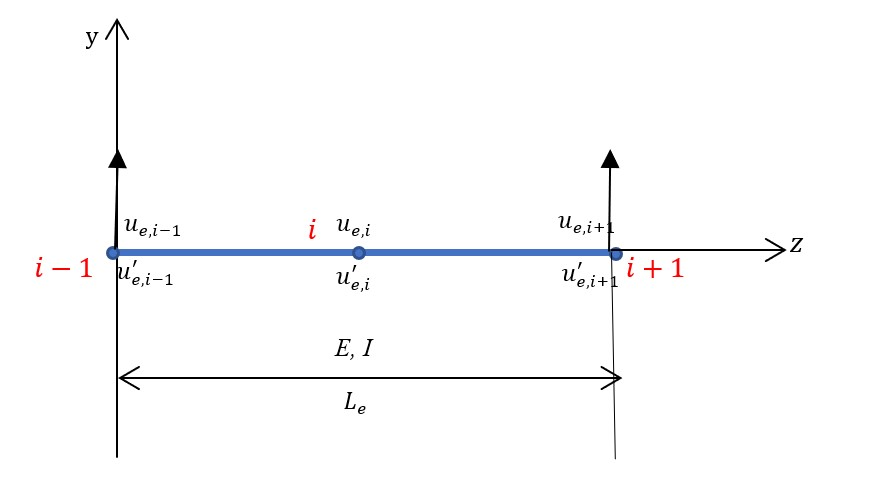
\includegraphics[width=\textwidth]{threedot}
				\caption{Трёхузловой конечный элемент}
				\label{fig:threedot}
			\end{figure}
		\end{column}
		\begin{column}{0.58\textwidth}
			\begin{figure}[H]
				\centering
				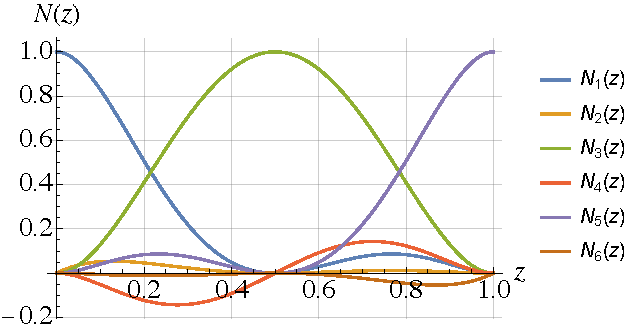
\includegraphics[width=\textwidth]{3_formfunctions.pdf}
				\caption{Функции формы для трёхузлового конечного элемента длиной $L_{e}=1$}
				\label{fig:3_formfunctions}
			\end{figure}
		\end{column}
	\end{columns}
\end{frame}

\begin{frame}
	\begin{block}{Функции формы для трёхузлового конечного элемента:}
			\begin{columns}
				\begin{column}{0.5\textwidth}
					\[
						\Scale[0.65]{
							\begin{split}
								N_{1e}(z)&=\frac{4}{L_{e}^{5}}\left(z-\frac{L_{e}}{2}\right)^{2}(z-L_{e})^{2}(L_e+6 z) \\
								N_{2e}(z)&=\frac{z (L_{e}-2 z)^2 (L_{e}-z)^2}{L^4}, \\
								N_{3e}(z)&=\frac{16 z^2 \left(z-L_e\right){}^2}{L_e^4},\\							
							\end{split}
						}
					\]
				\end{column}
				\begin{column}{0.5\textwidth}
					\[
						\Scale[0.65]{
							\begin{split}
								N_{4e}(z)&=\frac{8 z^2 \left(z-L_e\right){}^2 \left(2 z-L_e\right)}{L_e^4}, \\
								N_{5e}(z)&=-\frac{z^2 \left(6 z-7 L_e\right) \left(L_e-2 z\right){}^2}{L_e^5}, \\
								N_{6e}(z)&=\frac{z^2 \left(z-L_e\right) \left(L_e-2 z\right){}^2}{L_e^4}.
							\end{split}
						}
					\]
				\end{column}
			\end{columns}
	\end{block}
	\begin{block}{Матрица жесткости для трехузлового элемента:}
		\begin{equation*}
			\Scale[0.9] {
				\textbf{K}_e=\frac{EI}{L_e^{3}}
				\left[
				\begin{array}{cccccc}
					\frac{5092}{35} & \frac{1138 L_e}{35} & -\frac{512}{5} & \frac{384 L_e}{7} & -\frac{1508}{35}& \frac{242 L_{e}}{35}\\
						\frac{1138 L_{e}}{35} & \frac{332 L_e^{2}}{35} & -\frac{128 L_e}{5} & \frac{64 L_e^{2}}{7} & -\frac{242 L_{e}}{35}& \frac{38 L_{e}^{2}}{35}\\
					-\frac{512}{5} & -\frac{128 L_e}{5} & -\frac{1024}{5} & 0 & -\frac{512}{5}& \frac{128  L_{e}}{5}\\
						\frac{384 L_{e}}{7} & \frac{64 L_e^{2}}{7} & 0 & \frac{256 L_e^{2}}{7} & -\frac{384 L_{e}}{7}& \frac{64 L_{e}^{2}}{7}\\
					-\frac{1508}{35} & -\frac{242 L_e}{35} & -\frac{512}{5} & -\frac{384 L_{e}}{7} & \frac{5092}{35} &  -\frac{1138  L_{e}}{35}\\
						\frac{242 L_{e}}{35} & \frac{38 L_e^{2}}{35} &  \frac{128 L_e}{5} & \frac{64 L_e^{2}}{7} & -\frac{1138 L_{e}}{35}& \frac{332 L_{e}^{2}}{35}\\
				\end{array}
				\right]
			}
		\end{equation*}
	\end{block}
\end{frame}

\begin{frame}{}
	\begin{block}{Уравнение, описывающее прогиб упругой линии балки}
	$$(EIy^{''}_{zz})^{''}_{zz}=q,$$\\
где  $q$ -- функция внешней нагрузки.
	\end{block}
	\begin{figure}[H]
		\centering
		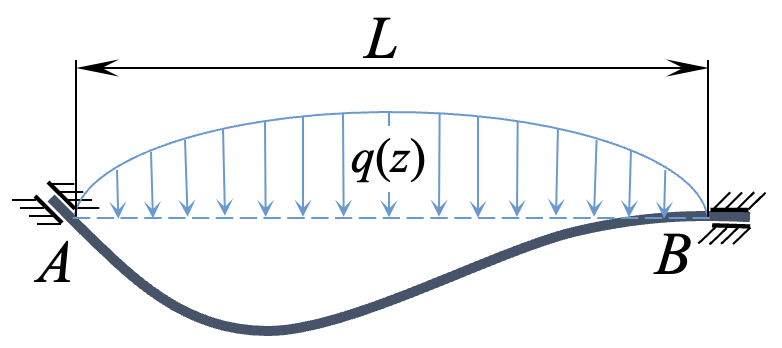
\includegraphics[width=0.5\textwidth]{beam}
		\label{fig:beam}
		\caption{Балка длиной $L=1$ под действием гладкой внешней нагрузки}
	\end{figure}
Граничные условия:
\begin{enumerate} 
	\item $y|_{z=0}=0$ -- отсутствие перемещения в т.$A$;\\
	\item $y^{'}|_{z=0}=-\frac{\pi}{180}$ -- поворот в т.$A$ на $1^{\circ};$\\
	\item $y|_{z=L}=0$ -- отсутствие перемещения в т.$B$;\\ 
	\item $y^{'}|_{z=L}=0$ -- отсутствие поворота сечения в т.$B$.\\
\end{enumerate}
\end{frame}

\begin{frame}{Гладкая функция внешней нагрузки:}
	\begin{block}{Гладкая функция внешней нагрузки:}
		\[q=-\frac{Q}{L} \sin(\pi z).\]
	\end{block}

	\begin{figure}[H]
		\centering
		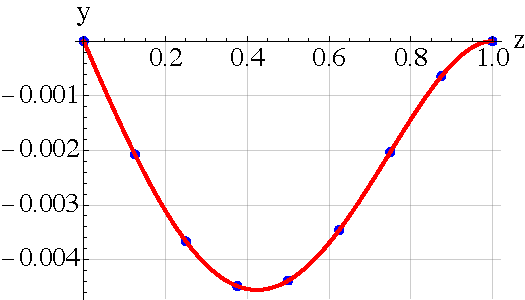
\includegraphics[width=0.75\textwidth]{3_comparison}
		\caption{Сравнение точного и приближенного решения при $n=4$, полученного при помощи МКЭ}
		\label{fig:3_comparison}
	\end{figure}
\end{frame}


\begin{frame}{}
	\begin{columns}
		\begin{column}{0.57\textwidth}
			\begin{figure}[H]
				\centering
				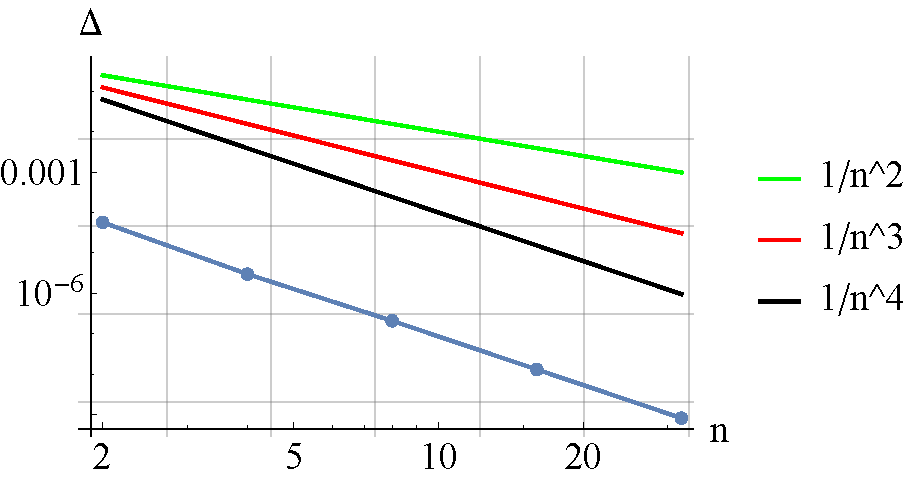
\includegraphics[width=\textwidth]{2_nodebeam_plain}
				\caption{Зависимость погрешности от числа конечных элементов (двухузловой КЭ)}
				\label{2_nodebeam_plain}
			\end{figure}
		\end{column}
		\begin{column}{0.57\textwidth}
			\begin{figure}[H]
				\centering
				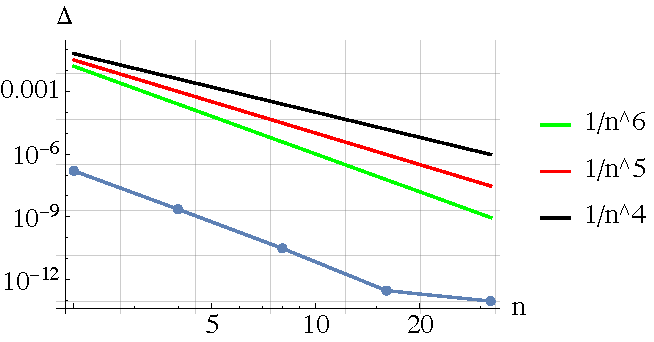
\includegraphics[width=\textwidth]{3_nodebeam_plain}
				\caption{Зависимость погрешности от числа конечных элементов (трехузловой КЭ)}
				\label{3_nodebeam_plain}
			\end{figure}
		\end{column}
	\end{columns}
	\begin{columns}
		\begin{column}{0.5\textwidth}
			\[
				\Scale[0.5] {
					\begin{array}{|c|c|c|c|c|c|}
							\hline
							\text{N} & 2 & 4 & 8 & 16 & 32 \\ \hline
							\Delta  & 5.87 \cdot 10^{-5}  & 3.51 \cdot 10^{-9} & 2.17 \cdot 10^{-7} & 1.35 \cdot 10^{-8} & 8.43 \cdot 10^{-10}\\ \hline
							m &  & 4.06 & 4.02 & 4.1 & 4.01 \\ 
							\hline
					\end{array}
				}
			\]
		\end{column}
		\begin{column}{0.5\textwidth}
			\[
				\Scale[0.5] {
					\begin{array}{|c|c|c|c|c|c|}
							\hline
							\text{N} & 2 & 4 & 8 & 16 & 32 \\ \hline
							\Delta  & 1.56 \cdot 10^{-7} & 2.31 \cdot 10^{-9} & 3.13 \cdot 10^{-11} & 3.01 \cdot 10^{-13} & 9.36 \cdot 10^{-14} \\ \hline
							m &  & 6.08 & 6.21 & 6.71 & 1.68 \\ 
							\hline
					\end{array}
				}
			\]
		\end{column}
	\end{columns}
\end{frame}


\begin{frame}{}
	Непрерывная негладкая функция внешней нагрузки с "изломом" в узле:
	\begin{equation}
		q = 
			\begin{cases}
				Q \sin \left(\frac{\pi  z}{z_{0}}\right) & z \leq z_{0}, \\
				Q \sin \left(\frac{\pi  (z-z_{0})}{z_{0}}\right) & z > z_{0},
			\end{cases}
	\end{equation}
	где $z_{0}=\frac{L}{2}$ --- точка разрыва, $L$ --- длина балки. \\
	\begin{figure}[H]
		\centering
		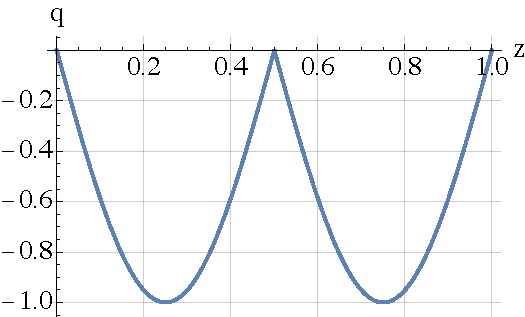
\includegraphics[width=0.5\textwidth]{q_cont_in}
		\caption{Непрерывная негладкая внешняя нагрузка $q$, действующая на балку}
		\label{fig:q_cont_in}
	\end{figure}
\end{frame}

\begin{frame}{}
	\begin{columns}
		\begin{column}{0.57\textwidth}
			\begin{figure}[H]
				\centering
				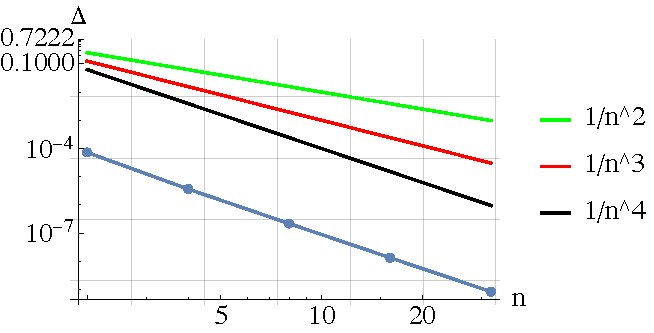
\includegraphics[width=0.99\textwidth]{2_nodebeam_cont_in}
				\caption{Зависимость погрешности от числа конечных элементов (двухузловой КЭ)}
				\label{fig:2_nodebeam_cont_in}
			\end{figure}
		\end{column}
		\begin{column}{0.57\textwidth}
			\begin{figure}[H]
				\centering
				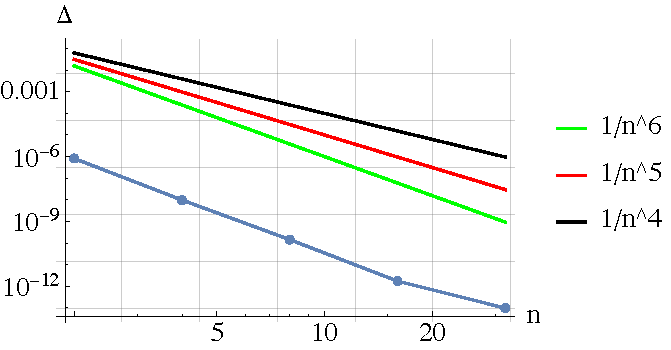
\includegraphics[width=0.9\textwidth]{3_nodebeam_cont_in}
				\caption{Зависимость погрешности от числа конечных элементов (трехузловой КЭ)}
				\label{fig:3_nodebeam_cont_in}
			\end{figure}
		\end{column}
	\end{columns}
	\begin{columns}
		\begin{column}{0.5\textwidth}
			\[
				\Scale[0.5] {
						\begin{array}{|c|c|c|c|c|c|}
								\hline
								\text{N} & 2 & 4 & 8 & 16 & 32 \\ \hline
								\Delta  & 7.21 \cdot 10^{-5} & 3.67 \cdot 10^{-6} & 2.21 \cdot 10^{-7} & 1.35 \cdot 10^{-8} & 8.44 \cdot 10^{-10}\\ \hline
								m  &  & 4.31 & 4.06 & 4.02 & 4.01 \\ 
								\hline
						\end{array}
				}
			\]
		\end{column}
		\begin{column}{0.5\textwidth}
			\[
				\Scale[0.5] {
					\begin{array}{|c|c|c|c|c|c|}
						\hline
						\text{N} & 2 & 4 & 8 & 16 & 32\\ \hline
						\Delta  & 8.16 \cdot 10^{-7} & 9.82 \cdot 10^{-9} & 1.45 \cdot 10^{-10} & 1.74 \cdot 10^{-12} & 9.82 \cdot 10^{-14}\\ \hline
						m &  & 6.38 & 6.08 & 6.38 & 4.14 \\ 
						\hline
					\end{array}
				}
			\]
		\end{column}
	\end{columns}
\end{frame}



\begin{frame}{}
	Непрерывная негладкая функция внешней нагрузки с "изломом" не в узле, т.е.
	$z_{0}=\frac{3L}{7}.$ 
	
	
	\begin{columns}
		\begin{column}{0.57\textwidth}
			\begin{figure}[H]
				\centering
				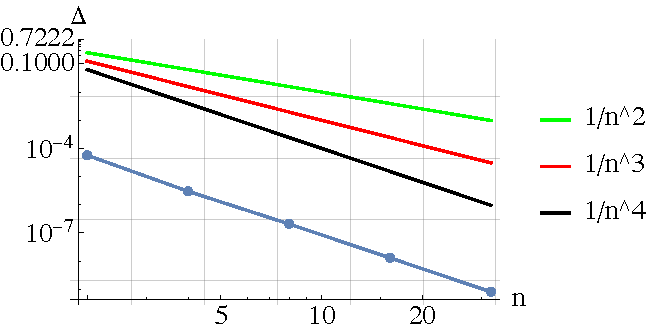
\includegraphics[width=0.99\textwidth]{2_nodebeam_cont_out}
				\caption{Зависимость погрешности от числа конечных элементов (двухузловой КЭ)}
				\label{fig:2_nodebeam_cont_out}
			\end{figure}
		\end{column}
		\begin{column}{0.57\textwidth}
			\begin{figure}[H]
				\centering
				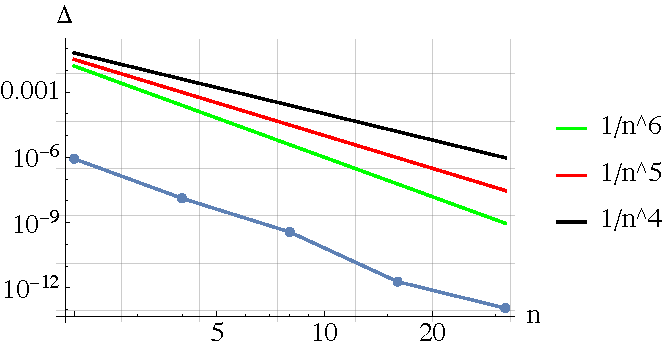
\includegraphics[width=0.9\textwidth]{3_nodebeam_cont_out}
				\caption{Зависимость погрешности от числа конечных элементов (трехузловой КЭ)}
				\label{fig:3_nodebeam_cont_out}
			\end{figure}
		\end{column}
	\end{columns}
	\begin{columns}
		\begin{column}{0.5\textwidth}
			\[
				\Scale[0.5] {
						\begin{array}{|c|c|c|c|c|c|}
								\hline
								\text{N} & 2 & 4 & 8 & 16 & 32 \\ \hline
								\Delta  & 5.7 \cdot 10^-7 & 3.11 \cdot 10^{-6} & 2.08 \cdot 10^{-7} & 1.32 \cdot 10^{-8} & 8.11 \cdot 10^{-10}\\ \hline
								m  &  &4.25 & 3.85 & 3.90 & 4.01 \\ 
								\hline
								\end{array}
				}
			\]
		\end{column}
		\begin{column}{0.5\textwidth}
			\[
					\Scale[0.5] {
			\begin{array}{|c|c|c|c|c|c|}
			\hline
			\text{N} & 2 & 4 & 8 & 16 & 32 \\ \hline
			\Delta  & 8.55 \cdot 10^{-7} & 1.31 \cdot 10^{-8} & 3.70 \cdot 10^{-10} & 1.94 \cdot 10^{-12} & 1.18 \cdot 10^{-13}  \\ \hline
			m  & & 6.03 & 5.15 & 7.57 & 4.03 \text{} \\ 
			\hline
			\end{array}
				}
				\]
		\end{column}
	\end{columns}
\end{frame}


\begin{frame}
	\begin{block}{Ограниченная функция внешней нагрузки с "изломом" в узле}
		\begin{equation}
			\Scale[0.7]{q = 
			\begin{cases}
				Q \sin \left(\frac{\pi  z}{z_{0}}\right) & z \leq  z_{0}, \\
				Q \sin \left(\frac{\pi  (z-z_{0})}{z_{0}}\right) & z > z_{0},
			\end{cases}
			}
		\end{equation}
	\end{block}
	где $z_{0}=\frac{L}{2}$ --- точка разрыва производной, $L$ --- длина балки. \\

		\begin{columns}
			\begin{column}{0.57\textwidth}
				\begin{figure}[H]
					\centering
					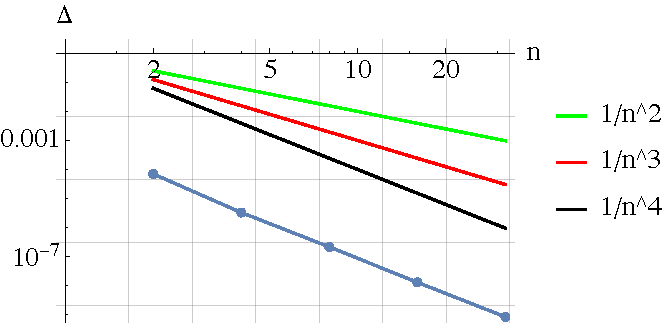
\includegraphics[width=0.99\textwidth]{2_nodebeam_cont_finite_in}
					\caption{Зависимость погрешности от числа конечных элементов (двухузловой КЭ)}
					\label{fig:2_nodebeam_cont_finite_in}
				\end{figure}
			\end{column}
			\begin{column}{0.57\textwidth}
				\begin{figure}[H]
					\centering
					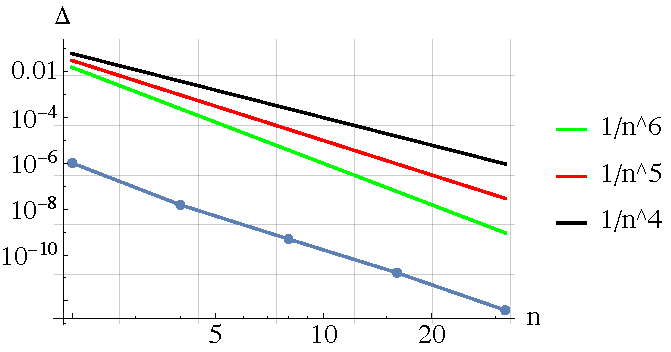
\includegraphics[width=0.9\textwidth]{3_nodebeam_cont_finite_in}
					\caption{Зависимость погрешности от числа конечных элементов (трехузловой КЭ)}
					\label{fig:3_nodebeam_cont_finite_in}
				\end{figure}
			\end{column}
		\end{columns}
		\begin{columns}
			\begin{column}{0.5\textwidth}
				\[
					\Scale[0.5] {
							\begin{array}{|c|c|c|c|c|c|}
									\hline
									\text{N} & 2 & 4 & 8 & 16 & 32 \\ \hline
			\Delta  & 7.11 \cdot 10^{-5} & 3.32 \cdot 10^{-6} & 2.20 \cdot 10^{-7} & 1.32 \cdot 10^{-8} & 8.42 \cdot 10^{-10}\\ \hline
			m  &  & 4.41 & 3.94 & 4.06 & 3.95 \\ 
									\hline
									\end{array}
					}
				\]
			\end{column}
			\begin{column}{0.5\textwidth}
				\[
						\Scale[0.5] {
				\begin{array}{|c|c|c|c|c|c|}
				\hline
				\text{N} & 2 & 4 & 8 & 16 & 32 \\ \hline
			\Delta  & 1.04 \cdot 10^{-6} & 1.55 \cdot 10^{-8} & 4.92 \cdot 10^{-10} & 1.69 \cdot 10^{-11} & 3.92 \cdot 10^{-13} \\ \hline
			m  &  & 6.07 & 4.96 & 4.88 & 5.43 \\ 
				\hline
				\end{array}
					}
					\]
			\end{column}
		\end{columns}
	\end{frame}




	\begin{frame}{}
		Ограниченная функция внешней нагрузки с "изломом" не узле
			\begin{columns}
				\begin{column}{0.57\textwidth}
					\begin{figure}[H]
						\centering
						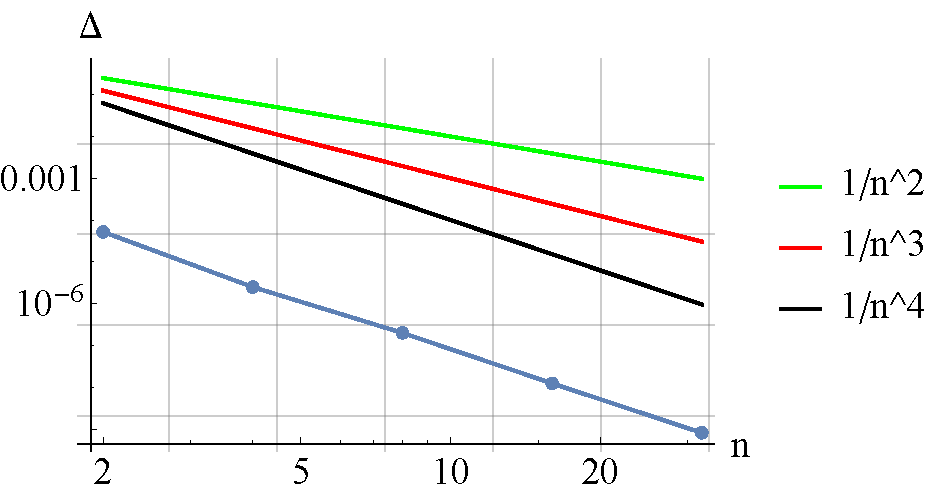
\includegraphics[width=0.99\textwidth]{2_nodebeam_cont_finite_out}
						\caption{Зависимость погрешности от числа конечных элементов (двухузловой КЭ)}
						\label{fig:2_nodebeam_cont_finite_out}
					\end{figure}
				\end{column}
				\begin{column}{0.57\textwidth}
					\begin{figure}[H]
						\centering
						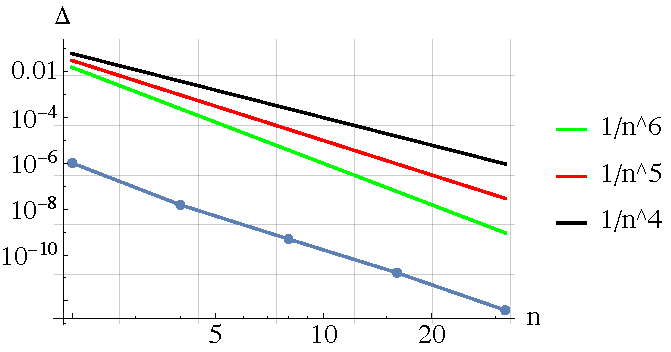
\includegraphics[width=0.99\textwidth]{3_nodebeam_cont_finite_out}
						\caption{Зависимость погрешности от числа конечных элементов (трехузловой КЭ)}
						\label{fig:3_nodebeam_cont_finite_out}
					\end{figure}
				\end{column}
			\end{columns}
			\begin{columns}
				\begin{column}{0.5\textwidth}
					\[
						\Scale[0.5] {
								\begin{array}{|c|c|c|c|c|c|}
									\hline
									\text{N} & 2 & 4 & 8 & 16 & 32 \\ \hline
									\Delta  & 5.21 \cdot 10^{-5} & 2.50 \cdot 10^{-6} & 1.92 \cdot 10^{-7} & 1.23 \cdot 10^{-8} & 8.12 \cdot 10^{-10} \\ \hline
									m  &  & 4.38 & 3.64 & 4.01 & 3.92 \\ 
									\hline
										\end{array}
						}
					\]
				\end{column}
				\begin{column}{0.5\textwidth}
					\[
							\Scale[0.5] {
					\begin{array}{|c|c|c|c|c|c|}
					\hline
					\text{N} & 2 & 4 & 8 & 16 & 32\\ \hline
				\Delta  & 1.02 \cdot 10^{-6} & 3.25 \cdot 10^{-8} & 5.93 \cdot 10^{-10} & 9.64 \cdot 10^{-12} & 1.39 \cdot 10^{-13}\\ \hline
				m  &  &  4.96 & 5.78 & 5.94 & 6.12 \\ 
					\hline
					\end{array}
						}
						\]
				\end{column}
			\end{columns}
		\end{frame}



	\begin{frame}{}
	\begin{block}{Сосредоточенная не в узле функция внешней нагрузки}
		\[q = 10 Q L  \delta (z - z_{0}),\]
	\end{block}
	где $z_{0}=\frac{3L}{7}$ --- точка разрыва производной, не совпадающая с узлом сетки, $\delta$ --- дельта-функция Дирака, $L=1$ --- длина балки. 
	\begin{columns}
		\begin{column}{0.57\textwidth}
			\begin{figure}[H]
				\centering
				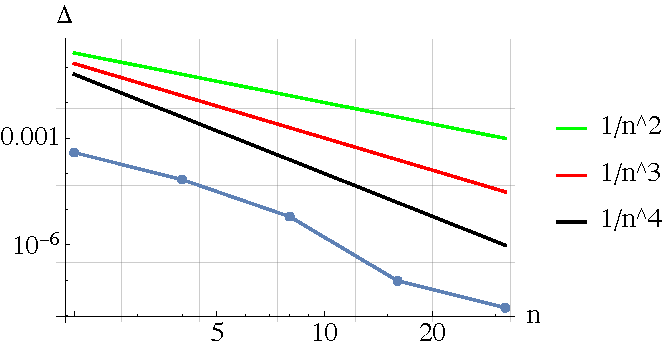
\includegraphics[width=0.8\textwidth]{2_nodebeam_concentrated_out}
				\caption{Зависимость погрешности от числа конечных элементов (двухузловой КЭ)}
				\label{fig:2_nodebeam_concentrated_out}
			\end{figure}
		\end{column}
		\begin{column}{0.57\textwidth}
			\begin{figure}[H]
				\centering
				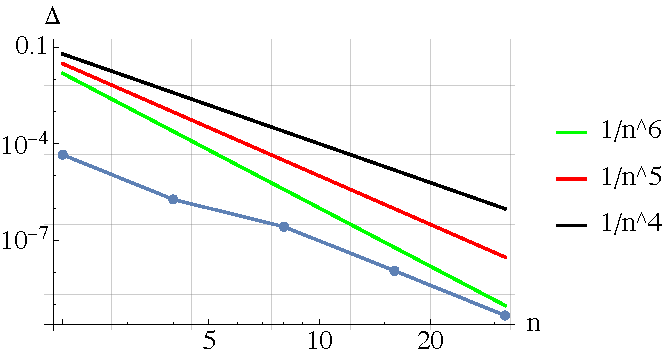
\includegraphics[width=0.8\textwidth]{3_nodebeam_concentrated_out}
				\caption{Зависимость погрешности от числа конечных элементов (трехузловой КЭ)}
				\label{fig:3_nodebeam_concentrated_out}
			\end{figure}
		\end{column}
	\end{columns}
	\begin{columns}
		\begin{column}{0.5\textwidth}
			\[
				\Scale[0.5] {
						\begin{array}{|c|c|c|c|c|c|}
							\hline
							\text{N} & 2 & 4 & 8 & 16 & 32\\ \hline
				\Delta  &3.91 \cdot 10^{-4} & 6.72 \cdot 10^{-5} & 6.11 \cdot 10^{-6} & 9.53 \cdot 10^{-8} & 1.65 \cdot 10^{-8} \\ \hline
				m  &  & 2.52 & 3.47 & 6.00 & 2.52 \\ 
							\hline
								\end{array}
				}
			\]
		\end{column}
		\begin{column}{0.5\textwidth}
			\[
					\Scale[0.5] {
			\begin{array}{|c|c|c|c|c|c|}
			\hline
			\text{N} & 2 & 4 & 8 & 16 & 32\\ \hline
				\Delta  & 4.52 \cdot 10^{-5} & 1.86 \cdot 10^{-6} & 2.64 \cdot 10^{-7} & 1.12 \cdot 10^{-8} & 4.54 \cdot 10^{-10} \\ \hline
				m  &  &  4.62 & 2.82 & 4.56 & 4.62 \\ 
			\hline
			\end{array}
				}
				\]
		\end{column}
	\end{columns}
\end{frame}

\end{document}
